\clearpage

\AddToShipoutPictureBG{
    \begin{tikzpicture}[remember picture, overlay]
        \node[opacity=0.08] at (current page.center) {
            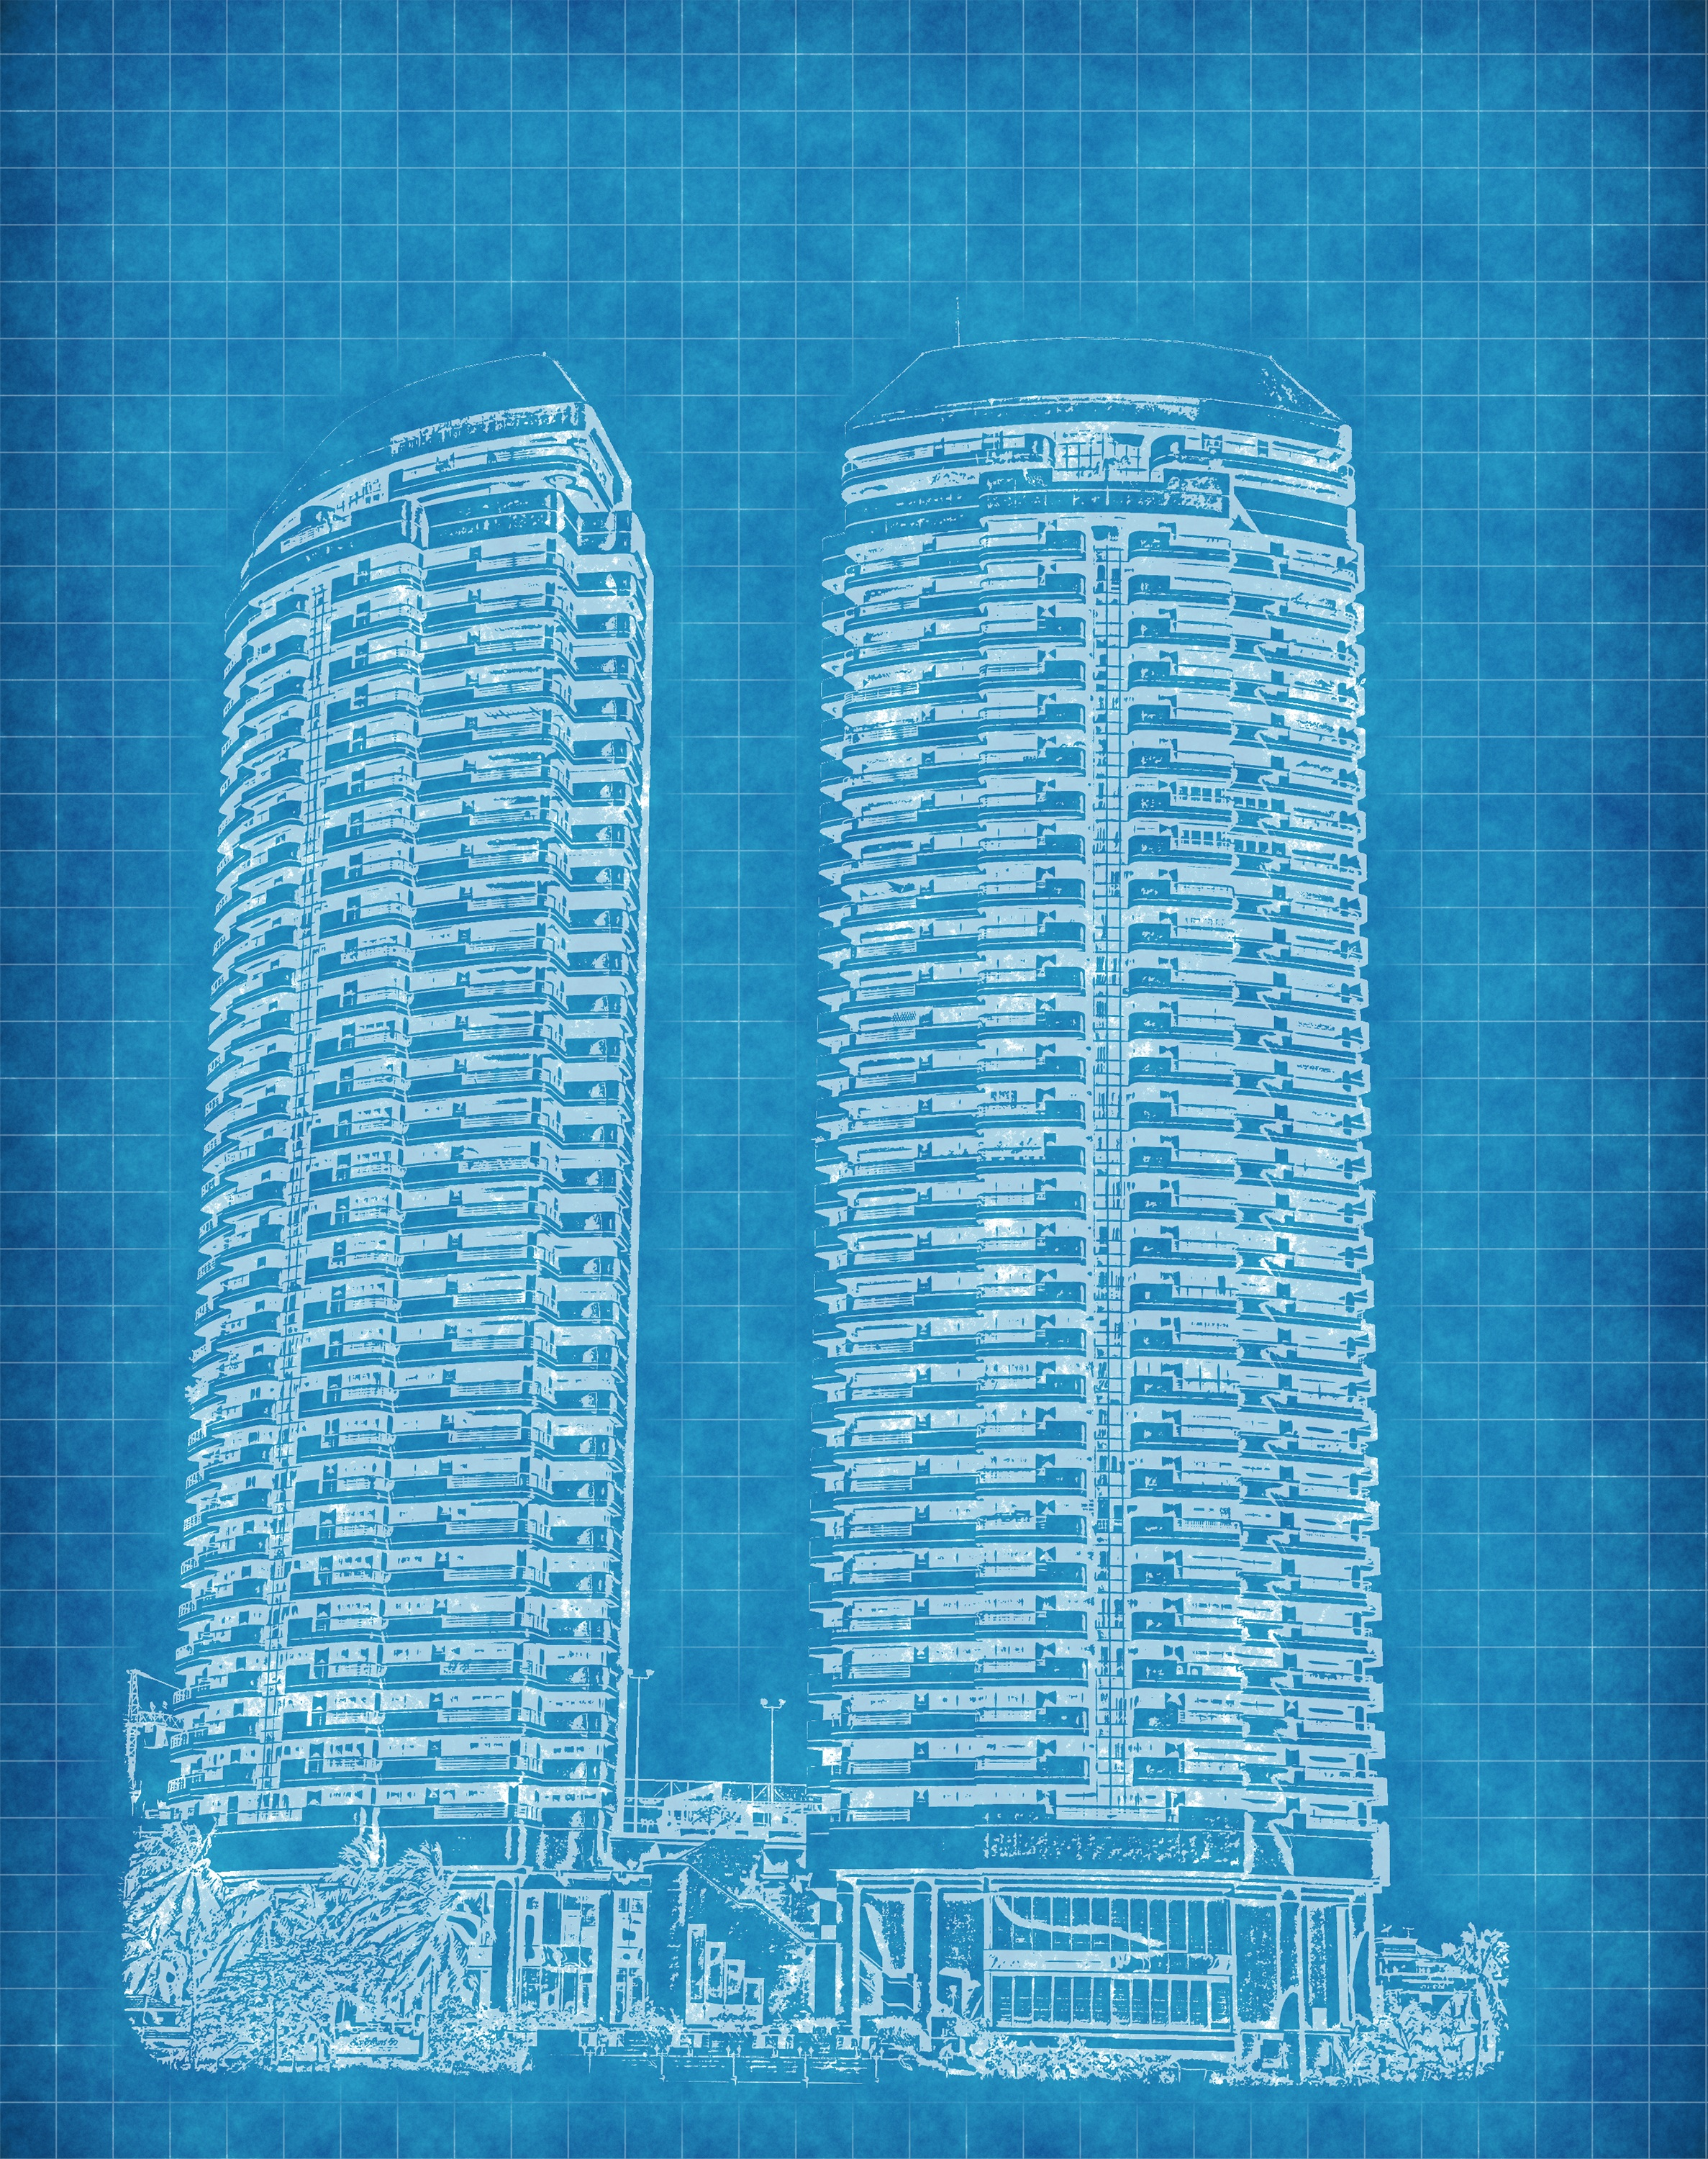
\includegraphics[width=\paperwidth,height=\paperheight]{image/blueprint}
        };
    \end{tikzpicture}
}

\chapter{But du portfolio}
\label{chap:but_portfolio}

\section{Cadre formel et ancrage théorique}

Le présent portfolio d'apprentissage s'érige dans le cadre du Master HES-SO Innokick, au sein du module de Différenciation Métier (MDM), en vue de la validation des 6 crédits ECTS qui lui sont associés. Ce travail a été échafaudé sous la supervision de Bastien Petitpierre, professeur référent, durant l'année académique 2025-2026.

\subsection*{Question structurante du portfolio}

Le présent travail s'organise autour d'une question unique, formulée en début de rédaction et tenue tout au long du document :

\begin{quote}
\itshape
Comment un ingénieur logiciel, formé à la résolution technique de problèmes, peut-il documenter avec rigueur le développement de compétences situées \emph{au-delà du code}, et démontrer leur mobilisation effective dans des situations professionnelles complexes ?
\end{quote}

Cette question oriente trois choix structurants : la sélection délibérée de trois compétences (A2, B4, C2) dont le développement marque la rupture la plus nette avec le profil initial ; la mobilisation d'un terrain professionnel dense (TWIICE, dispositifs médicaux certifiés) susceptible de produire des traces auditables ; et l'adoption stricte du cadre Tardif comme grille d'évaluation des preuves. Le référentiel auquel se rattachent ces trois compétences, ainsi que le module dans lequel s'inscrit le présent travail, sont introduits ultérieurement, au chapitre~\ref{chap:pec_documents} (\emph{Repères institutionnels}) ; leur justification détaillée est conduite, quant à elle, à la section~\ref{sec:trois-competences-justification}. Chacun des chapitres qui suivent peut être lu comme une instruction partielle de cette question.

\citet{tardif2006} définit le portfolio d'apprentissage en ces termes :

\begin{quote}
    « Un échantillon de preuves, sélectionnées par l'élève ou par l'étudiant dans l'intention de rendre compte fidèlement des apprentissages réalisés au cours d'une période ou au terme de cette période, qui fournit les données nécessaires, celles-ci comprenant une autoévaluation, pour que soit porté un jugement judicieux et éthique sur le niveau de développement des compétences concernées, sur le degré de maîtrise des ressources pouvant être mobilisées et combinées, ainsi que sur l'étendue des situations dans lesquelles ce niveau de développement et ce degré de maîtrise sont susceptibles de se matérialiser. » \citep[p.~266]{tardif2006}
\end{quote}

Il ne s'agit donc pas d'un simple assemblage de documents, mais bien d'un récit étayé par des preuves, rendant compte d'une progression dans les apprentissages. L'étudiant que je suis, est appelé à identifier ses ressources, à démontrer la manière dont il les agence au sein de situations concrètes, et à porter un regard autoévaluatif sur son propre développement. Cette démarche s'inscrit dans le prolongement d'une pratique réflexive, telle que la conçoivent \citet{lafortune2001} :

\begin{quote}
    « C'est là ce que peut faire le praticien réflexif, c'est-à-dire, une personne capable de décrire et d'analyser sa pratique afin de la rendre plus efficace et de développer ses propres modèles d'intervention. » \citep[p.~68]{lafortune2001}
\end{quote}

C'est précisément sur ces deux piliers, documentaire et réflexif, que le présent portfolio a été bâti. Les sections qui suivent exposent successivement les fondations professionnelles antérieures à la formation, les objectifs poursuivis et la posture réflexive adoptée tout au long de la démarche.

\subsection*{Note méthodologique et choix de structure}

\textbf{Recours à l'intelligence artificielle.}
Ce document a été rédigé avec l'assistance de l'intelligence artificielle (principalement des modèles de génération de texte de type grand modèle de langage), utilisée comme appui d'échafaudage, de reformulation et de clarification. Cette démarche s'inscrit explicitement dans le respect de deux cadres de référence : d'une part, les principes directeurs pour une bonne administration de l'IA générative dans l'enseignement définis par la HES-SO \citep{hessoIA2025}, qui encadrent les conditions d'un usage académique légitime et transparent au sein de l'institution ; d'autre part, la Recommandation sur l'éthique de l'intelligence artificielle proposée par l'UNESCO \citep{unescoIA2022}, qui pose les principes fondamentaux d'un recours responsable, centré sur la dignité humaine, la transparence et la redevabilité. Concrètement, l'IA a été mobilisée pour dresser les plans de sections, consolider la formulation de passages complexes, vérifier la solidité des enchaînements argumentatifs et poser des pierres d'appui là où l'expression manquait de charpente. Dans tous les cas, les idées, les expériences relatées, les preuves sélectionnées ainsi que les liens établis avec le référentiel de compétences sont le fruit d'un travail d'analyse personnelle. L'IA n'a pas bâti le contenu à ma place : elle a agi comme un outil d'assistance à la mise en forme, de la même manière qu'un traitement de texte ou un correcteur orthographique soutient la rédaction sans s'y substituer.

\textbf{Choix de la structure du document.}
La structure de ce portfolio n'a pas été imposée strictement par le cadre pédagogique : elle résulte d'un choix délibéré, visant à bâtir une architecture cohérente entre les différentes dimensions de la démarche. Le document se déploie en sept chapitres, regroupés en quatre ensembles de lecture.

\begin{itemize}
    \item \textbf{Un socle d'ouverture} pose les fondations : le chapitre \emph{But du portfolio} expose le cadre formel, l'ancrage théorique, le profil initial et les objectifs poursuivis ; le chapitre \emph{Titre du portfolio} explicite le sens du titre retenu et la logique symbolique qui soutient l'ensemble du document ; le chapitre \emph{Contrat individuel d'apprentissage} formalise les engagements posés en début de formation.

    \item \textbf{Un seuil de cadrage institutionnel}, constitué du chapitre \emph{Repères institutionnels}, dont le rôle est délibérément liminaire : rappeler succinctement les textes de référence (PEC, descriptif MDM, document cadre) sans y développer d'analyse substantielle.

    \item \textbf{Le cœur démonstratif du portfolio} se déploie ensuite en deux strates complémentaires. \emph{Espace modules} assure une fonction de cartographie : il rend visibles les apprentissages, les ressources rencontrées et leur mise en perspective. \emph{Situations professionnalisantes et analyse des compétences} remplit une fonction probatoire : il documente, avec situations, traces et preuves détaillées, la démonstration des compétences A2, B4 et C2.

    \item \textbf{Un horizon d'ouverture}, enfin, constitué du chapitre \emph{Perspectives pour la suite}, ouvre le chantier des prolongements envisagés.
\end{itemize}

Cette architecture vise à donner à lire non seulement ce que j'ai appris, mais la trajectoire par laquelle ces apprentissages ont été construits.

Par ailleurs, afin de pallier une contrainte récurrente de la formation, à savoir la disponibilité parfois différée des supports de présentation des enseignants, j'ai fait le choix de décrire les ressources mobilisées ou de les reconstituer moi-même lorsque nécessaire. Ce choix reflète ma réalité d'apprentissage durant les cours : dans plusieurs situations, les supports étant transmis a posteriori, la compréhension s'est d'abord construite à partir de mes notes.

\section{Note méthodologique}
\label{sec:note-methodologique}

Cette section explicite les choix méthodologiques qui structurent le portfolio, conformément à l'attente d'un travail académique de niveau Master : critères de sélection, modes de production des preuves, traitement des biais.

\subsection*{Sélection des trois compétences}

Le module de Différenciation Métier, dont le cadre est présenté au chapitre~\ref{chap:pec_documents} (\emph{Repères institutionnels}), impose la sélection de trois compétences au sein du référentiel Innokick (une par famille A, B, C), lui-même introduit dans ce même chapitre. Trois critères ont guidé la sélection retenue (A2, B4, C2) :

\begin{enumerate}
    \item \textbf{Critère d'écart au profil initial.} La compétence retenue devait correspondre à une zone clairement sous-développée dans le profil d'ingénieur logiciel d'entrée en formation. Les compétences déjà bien établies (par exemple B6 \emph{Élaboration de roadmaps}, ancrée dans l'expérience professionnelle antérieure) ont été écartées, car elles n'auraient pas permis de documenter une \emph{progression}.
    \item \textbf{Critère de mobilisation effective.} La compétence devait avoir été réellement sollicitée dans une situation professionnelle complexe au cours de l'année, et avoir produit des artefacts datés susceptibles d'être interprétés comme preuves au sens de~\citet{tardif2006}.
    \item \textbf{Critère de cohérence d'ensemble.} Les trois compétences retenues devaient former un système cohérent, en convergeant vers une posture professionnelle identifiable (ici : architecture décisionnelle, à l'interface du technique et du stratégique).
\end{enumerate}

\subsection*{Sélection des situations professionnalisantes et des artefacts}

Pour chaque compétence retenue, une situation professionnelle principale a été choisie selon trois critères : (i) authenticité (situation réellement vécue, non simulée) ; (ii) complexité (présence d'une divergence ou d'un arbitrage non trivial) ; (iii) traçabilité (production d'au moins un artefact daté et auditable). L'encart d'authenticité en tête du chapitre \emph{Situations professionnalisantes et analyse des compétences} précise, pour chaque artefact mobilisé, sa date de production, son contexte d'origine, sa version et son statut.

Une situation secondaire \emph{intra-Innokick} (atelier de prototypage en groupe) est mobilisée pour la compétence A2 afin d'éprouver la \emph{transférabilité} du développement de cette compétence hors du terrain principal TWIICE.

\subsection*{Mode de production des autoévaluations chiffrées}

Les scores avant/après formation (radars du \emph{Bilan de progression}) sont des autoévaluations \emph{reconstituées a posteriori}, calibrées sur la grille de descripteurs Tardif (\emph{découvrir → appliquer → mobiliser → transmettre}, reproduite en tête du bilan). Trois précautions méthodologiques sont assumées :

\begin{itemize}
    \item Les scores « avant » n'ont pas été produits en début d'année puis archivés : ils sont une lecture réflexive de l'écart parcouru, non une mesure indépendante du temps t-0. Cette limite est explicitement documentée dans le chapitre dédié.
    \item Les scores « après » sont ancrés, dans la mesure du possible, à des artefacts vérifiables (preuves probatoires mobilisées dans le chapitre \emph{Situations}).
    \item Aucune triangulation par un tiers (pair, enseignant, hiérarchie) n'est intégrée au corps du portfolio ; les sources de triangulation externes disponibles (historique GitLab, comptes-rendus signés, validations hiérarchiques) sont listées en tête du chapitre \emph{Situations} et communicables à l'examinateur sur demande motivée.
\end{itemize}

\subsection*{Traitement des biais et des limites}

Quatre biais sont explicitement assumés dans ce travail :

\begin{itemize}
    \item \textbf{Biais rétrospectif} des scores « avant », typique des autoévaluations a posteriori (cf.~encart dédié dans le \emph{Bilan de progression}).
    \item \textbf{Concentration sur un terrain unique (TWIICE)} pour deux des trois compétences (B4 et C2). Cette limite est posée comme constat ; elle est partiellement compensée par l'introduction d'un second contexte pour A2 (atelier prototypage Innokick).
    \item \textbf{Pivot rétrospectif du 3\textsuperscript{e} critère du contrat d'apprentissage} (design / lecture de marché -> \emph{couche de pilotage orientée valeur} [\textit{business layer}]), documenté et argumenté dans le chapitre \emph{Perspectives}, mais sans note de pivot horodatée en cours d'année (cf.~annexe dédiée).
    \item \textbf{Usage de l'intelligence artificielle générative} dans la rédaction, déclaré dans la sous-section précédente et instrumenté en annexe~\ref{annex:usage-ia} (modèles, périmètre d'usage, périmètre d'exclusion, dispositif de vérification).
\end{itemize}

Ces biais ne sont pas considérés comme des défauts à dissimuler, mais comme des éléments constitutifs du dispositif méthodologique : leur explicitation participe de l'exigence de probité attendue d'un travail réflexif au sens de~\citet{schon1994} et~\citet{perrenoud2001}.

\section{Ancrage professionnel initial}

Ingénieur logiciel\footnote{Un \textbf{ingénieur logiciel} est un professionnel qui conçoit, développe, teste, déploie et maintient des \textbf{logiciels} : c'est-à-dire des programmes informatiques (suites d'instructions exécutées par une machine) destinés à automatiser une tâche, traiter de l'information ou piloter un système. À la différence du simple développeur, l'ingénieur logiciel applique une démarche \textbf{d'ingénieur} : analyse formelle d'un besoin, choix raisonné d'une architecture, prise en compte des contraintes de fiabilité, de performance, de sécurité et de coût, et capacité à justifier ses décisions techniques. Le terme « ingénieur » désigne ici plus largement un professionnel formé à résoudre des problèmes complexes par une approche méthodique et quantifiée, en s'appuyant sur des connaissances scientifiques et des standards reconnus.\label{fn:ingenieur-logiciel}} de formation, diplômé de la Haute École d'Ingénierie et de Gestion du Canton de Vaud (HEIG-VD\footnote{La \textbf{HEIG-VD} (Haute École d'Ingénierie et de Gestion du Canton de Vaud) est une école d'ingénieurs et de gestion membre de la HES-SO, située à Yverdon-les-Bains. Elle délivre notamment des Bachelors of Science HES-SO en ingénierie (informatique, électricité, microtechnique, etc.) et en économie d'entreprise.}), mon parcours professionnel s'est édifié à travers plusieurs secteurs qui ont chacun posé une pierre à ma posture actuelle.

J'ai d'abord exercé dans le secteur industriel, où j'ai été chargé d'automatiser la récolte de données d'une chaîne de production. Cette expérience m'a ancré dans les réalités opérationnelles du terrain : contraintes de cadence, fiabilité des systèmes, nécessité d'architecturer\footnote{Le verbe \emph{architecturer}, employé ici dans son acception technique, désigne l'acte de concevoir et d'organiser structurellement un système logiciel ou matériel : définir ses composants, leurs responsabilités et leurs interactions de manière cohérente, robuste et évolutive.} des solutions robustes et immédiatement exploitables. Elle m'a également sensibilisé aux enjeux de communication entre les équipes techniques et les opérateurs de production.

J'ai ensuite intégré le secteur bancaire, au sein du département reporting\footnote{Le \emph{département reporting} d'une banque privée est chargé de produire les rapports financiers réglementaires et commerciaux destinés aux clients, aux régulateurs et à la direction : relevés de portefeuille, rapports de performance, déclarations fiscales et documents de conformité. Il opère à l'intersection des contraintes légales, des exigences des autorités de surveillance (FINMA, en contexte suisse) et des attentes des clients fortunés.\label{fn:reporting}} d'une banque privée. Dans cet environnement, j'ai été confronté aux enjeux de conformité réglementaire, à la coordination entre entités géographiquement distribuées et à la nécessité de produire des livrables\footnote{Un \textbf{livrable} (\emph{deliverable}) désigne tout produit, document ou artefact formellement remis à un destinataire (client, partie prenante, autorité réglementaire) au terme d'une activité ou d'un jalon de projet. En contexte logiciel et d'ingénierie, un livrable peut être un programme exécutable, un rapport, une spécification, un plan de tests, un dossier de conformité, etc. Il est généralement défini par un cahier des charges, soumis à des critères d'acceptation et tracé jusqu'à sa validation.\label{fn:livrable}} fiables sous contraintes strictes de présentation et de légalité. C'est dans ce contexte que j'ai perçu, pour la première fois, les fissures d'une approche exclusivement technique : mes propositions d'amélioration, bien que pertinentes sur le plan opérationnel, manquaient de charpente et de capacité de conviction auprès des parties prenantes.

J'ai également évolué brièvement dans l'industrie des systèmes audiovisuels, où je développais des interfaces de pilotage pour des équipements techniques. Bien que de courte durée, cette expérience m'a révélé l'importance cruciale de la compréhension des besoins utilisateurs en amont du développement. J'y ai posé les premières pierres, de manière empirique et sans plan méthodologique formel, d'une pratique du prototypage et de la validation par l'usage.

J'exerce désormais au sein de TWIICE, entreprise spécialisée dans la conception de dispositifs robotiques à visée médicale. Mes responsabilités portent principalement sur le développement des différents logiciels embarqués\footnote{Dans ce contexte, les \emph{logiciels embarqués} désignent les programmes s'exécutant directement sur les composants matériels de l'exosquelette (microcontrôleurs, processeurs embarqués). Ils sont responsables du pilotage en temps réel des actionneurs, de l'acquisition des données issues des capteurs, de la gestion de l'alimentation ainsi que de la communication entre les différents modules électroniques du dispositif médical, par contraste avec les logiciels tournant sur des serveurs distants ou des applications mobiles.}, l'architecture\footnote{Le terme \emph{architecture}, employé ici dans son acception informatique, désigne l'organisation structurelle du système logiciel : la manière dont les différents composants logiciels sont découpés, agencés et mis en relation, ainsi que les décisions techniques qui régissent leurs interactions (protocoles de communication, interfaces, gestion des états). Dans le contexte de TWIICE, cela recouvre notamment la définition des flux de données entre le calculateur central, les cartes de contrôle moteur et l'interface utilisateur embarquée.} des communications entre eux ainsi que la mise en œuvre des conformités normatives en vigueur (IEC~62304\footnote{L'\emph{IEC~62304} \citep{iec62304} est une norme internationale qui définit les exigences relatives aux processus du cycle de vie des logiciels de dispositifs médicaux : développement, maintenance, gestion des risques logiciels et traçabilité. Elle est obligatoire pour tout logiciel intégré dans un dispositif médical mis sur le marché européen.\label{fn:iec62304}}, MDR\footnote{Le \emph{MDR} (\textit{Medical Device Regulation}, \citealp{mdr2017}) est le règlement européen sur les dispositifs médicaux, entré en application en mai 2021. Il remplace la directive MDD et renforce les exigences en matière de sécurité, de performance clinique, de surveillance post-marché et de traçabilité des dispositifs médicaux commercialisés dans l'Union européenne.}). Ce contexte, à la fois techniquement exigeant et fortement réglementé, a consolidé l'édifice de mon autonomie professionnelle.

C'est la convergence de ces expériences qui m'a conduit à un constat récurrent : il existe, entre l'étage technique dans lequel j'évolue avec aisance et l'étage métier où se décident la vision, la stratégie et la valeur d'un projet, un plafond de verre\footnote{\textbf{Note terminologique.} L'expression \emph{plafond de verre} (\textit{glass ceiling}) désigne, dans la littérature sociologique anglo-saxonne depuis les années 1980, les barrières invisibles qui freinent l'accès des femmes et des minorités aux positions de direction. L'emploi qui en est fait ici constitue un \emph{déplacement métaphorique assumé} vers la sphère des barrières de compétence personnelle : je conserve le mot pour son économie d'image (limite invisible mais étanche), tout en reconnaissant qu'il ne désigne pas, dans le présent portfolio, le concept sociologique d'origine. Le lecteur pourra y lire, plus précisément, un \emph{plafond de compétence transdisciplinaire}.\label{fn:plafond-verre}}. Je suis capable de concevoir, de développer et de livrer des solutions techniques robustes, mais je me heurte systématiquement à cette cloison invisible dès qu'il s'agit de contribuer pleinement au projet dans sa dimension globale.

Dans l'industrie, je pouvais automatiser une chaîne de production, mais je n'avais pas les clés pour défendre la valeur ajoutée de cette automatisation auprès de la direction. En banque, mes propositions d'amélioration étaient techniquement solides, mais elles ne franchissaient pas le seuil de la décision, faute de savoir les charpenter et les présenter de manière convaincante. Dans l'audiovisuel, j'ai entrevu l'importance du prototypage et de l'empathie utilisateur, sans disposer des plans méthodologiques pour formaliser cette intuition.

Ce plafond se manifeste toujours par les mêmes brèches dans mon profil : la capacité à concevoir des interfaces intelligibles et désirables, l'analyse de marché permettant d'identifier les besoins et les opportunités, l'aptitude à présenter et à défendre un projet de manière convaincante, ainsi que la compétence à déléguer et à collaborer au sein d'une équipe pluridisciplinaire. Sans ces compétences, je reste cloisonné dans le rôle d'exécutant technique, incapable de porter pleinement ma contribution à la création de valeur.

C'est cette prise de conscience, mûrie au fil de plusieurs années et de contextes professionnels variés, qui m'a conduit à m'engager dans la formation Innokick, avec l'intention de briser ce plafond et de bâtir une professionnalité plus complète.

\section{Objectifs du portfolio}

Conformément au cadre théorique posé par~\cite{tardif2006}, le présent portfolio vise à documenter l'élévation de ma trajectoire de développement à travers les six phases du Design Thinking (empathie, définition, idéation, prototypage, test, implémentation). De manière plus spécifique, il poursuit trois objectifs :

\begin{itemize}
    \item \textbf{Identifier les apprentissages érigés} au fil de chaque phase, en particulier dans des domaines éloignés de mon expertise initiale : la gestion des divergences et la facilitation collective (A2), la mise en œuvre de méthodes agiles dans un contexte réglementé (B4), ou encore la synthèse de problématiques complexes sous contrainte de certification (C2).
    \item \textbf{Rendre visibles les nouvelles ressources} progressivement maîtrisées : connaissances théoriques, méthodes (veille stratégique, prototypage, protocoles de validation), attitudes (ouverture, esprit critique), valeurs et schèmes d'action.
    \item \textbf{Démontrer l'assemblage et la combinaison de ces ressources} au sein de situations concrètes, qu'elles soient issues de la formation Innokick ou de mon contexte professionnel chez TWIICE.
\end{itemize}

Cette démarche illustre un parcours développemental structuré en trois niveaux : les fondations professionnelles acquises à l'entrée en formation, les transformations engagées en cours de cursus, et l'édifice professionnel visé à terme.

\section{Trois compétences, trois chantiers}
\label{sec:trois-competences-justification}

Le cadre académique du module de Différenciation Métier (MDM) du Master Innokick, dont la présentation détaillée fait l'objet du chapitre~\ref{chap:pec_documents} (\emph{Repères institutionnels}), impose une contrainte structurante : il ne s'agit pas de balayer l'intégralité des dix-huit compétences du référentiel Innokick, mais d'en \textbf{sélectionner trois}, une par famille, et d'en documenter le développement avec rigueur et profondeur. Les trois familles, dont le détail est également exposé au chapitre~\ref{chap:pec_documents}, sont les suivantes :

\begin{itemize}
    \item \textbf{Famille A} : Compétences sociales et personnelles
    \item \textbf{Famille B} : Compétences méthodologiques
    \item \textbf{Famille C} : Compétences métier
\end{itemize}

Ce choix n'est pas arbitraire. Il résulte d'une démarche réflexive : identifier, parmi les dix-huit compétences du référentiel, celles dont le développement illustre le mieux la rupture entre le profil que j'étais en entrant en formation et celui que j'ambitionne d'être. Chaque compétence retenue correspond à un étage structurant de cet édifice en construction, à un endroit précis où la formation a ébranlé une certitude, ouvert une brèche ou posé une poutre que l'intuition seule n'aurait pas suffi à dresser.

Les trois chantiers retenus sont :

\begin{description}
    \item[\textbf{A2 : Gestion des divergences et facilitation de la convergence}] \hfill \\
    Cette compétence incarne la rupture la plus profonde avec ma posture initiale d'ingénieur. Là où l'expert tend à trancher, à imposer une direction ou à défendre sa solution, le praticien compétent en A2 crée les conditions pour que le groupe converge par lui-même vers une décision partagée. Acquérir cette compétence, c'est ériger un étage entièrement nouveau : celui de la facilitation, de la médiation et de l'intelligence collective. C'est précisément là que se situe l'une des brèches les plus saillantes de mon profil initial, et c'est pourquoi ce chantier est au cœur de ce portfolio.

    \item[\textbf{B4 : Méthodes agiles au service du prototypage itératif}] \hfill \\
    Connaître une méthode est une chose ; savoir l'adapter à un contexte contraint en est une autre. La compétence B4 ne se réduit pas à la maîtrise de Scrum ou du Lean : elle exige de comprendre \emph{pourquoi} une méthode fonctionne, pour pouvoir la moduler quand le terrain impose ses propres contraintes. Pour un ingénieur qui aspire à dépasser le registre de l'exécution technique, cette capacité à piloter un processus itératif avec méthode et discernement constitue un pilier central de la professionnalité visée.

    \item[\textbf{C2 : Synthèse et définition des problématiques prioritaires}] \hfill \\
    La capacité à \emph{nommer le bon problème} avant de chercher une solution est l'une des marques les plus distinctives du professionnel de l'innovation. Cette compétence incarne le passage du technicien qui répond à la question posée au praticien qui s'assure d'abord que la bonne question est posée. Elle constitue la clé de voûte de l'édifice : sans une problématique bien définie, ni la créativité ni la rigueur méthodologique ne peuvent s'exercer pleinement.
\end{description}

\section{Le portfolio comme outil réflexif}

Au-delà de sa dimension certificative, ce portfolio constitue avant tout un instrument d'apprentissage et d'autorégulation. En conservant des traces structurées de mes réflexions, de mes réussites comme de mes difficultés, il me permet d'inspecter ma progression et d'ajuster ma démarche de manière continue.

Cette pratique réflexive s'appuie sur un questionnement métacognitif régulier, échafaudé autour des interrogations suivantes :

\begin{itemize}
    \item Quels savoirs ai-je acquis à travers ce cours, cette lecture, cette expérience ?
    \item En quoi ces apprentissages consolident-ils ou reconfigurent-ils ma manière de penser et d'agir ?
    \item Quelles conséquences en découlent sur ma façon de collaborer et d'exercer ma professionnalité ?
    \item Quels étages nouveaux vais-je ériger, et selon quelles modalités ?
\end{itemize}

Le portfolio se conçoit ainsi comme un chantier permanent d'interrogation de mes pratiques, de confrontation de mes intuitions aux cadres théoriques, et d'édification progressive d'une posture professionnelle qui s'élève au-delà du registre strictement technique.

\clearpage
\ClearShipoutPictureBG
